\documentclass{beamer}



\usepackage[ngerman]{babel}
\usepackage{default}
\usepackage[utf8]{inputenc}

\usepackage{amsmath}
\usepackage{amssymb}

\usetheme{Berlin}
\usecolortheme{beaver}
\uselanguage{ngerman}

\title{Korrespondenzproblem}
%\subtitle{Subtitle}
\author{Soeren Berken-Mersmann}
\institute
{
  DHBW Karlsruhe
}
\date{17. April 2015}
\subject{Theoretische Informatik}

\begin{document}
\frame{\titlepage}

\frame{
	\frametitle{Gliederung}
	
	\begin{enumerate}
		\item Postsches Korrespondenzproblem
		\item Simulation einer Turingmaschine
		\item Beweis der Nichtberechenbarkeit
		\item Beweise weiterer Probleme
	\end{enumerate}
}

\frame{
	\frametitle{Postsches Korrespondenzproblem}
	
	
	\[\begin{bmatrix}
		1 \\ 111
	\end{bmatrix}
	\begin{bmatrix}
		10111 \\ 10
	\end{bmatrix}
	\begin{bmatrix}
		10 \\ 0
	\end{bmatrix}\]
	\newline\newline
	Wer findet eine Reihenfolge, so dass unten und oben jeweils die gleiche Folge steht?
	\newline\newline
	\pause
	\[I_1 = (2, 1, 1, 3): 	\begin{bmatrix}
								10111 \\ 10
							\end{bmatrix} \begin{bmatrix}
								1 \\ 111
							\end{bmatrix} \begin{bmatrix}
								1 \\ 111
							\end{bmatrix} \begin{bmatrix}
								10 \\ 0
							\end{bmatrix}
	\]

}\frame{
	\[\begin{bmatrix}
		001 \\ 0
	\end{bmatrix}
	\begin{bmatrix}
		01 \\ 011
	\end{bmatrix}
	\begin{bmatrix}
		01 \\ 101
	\end{bmatrix}
	\begin{bmatrix}
		10 \\ 001
	\end{bmatrix}\]
	\newline\newline
	Wer findet hierfür eine Lösung?
	
	\pause
	
	\[I_1 = (2, 4, 3, 4, 4, 2, 1, 2, 4, 3, 4, 3, 4, 4, 3, 4, 4, 2, 1, 4, 4, 2, 1, 3, 4, 1, 1, 3,
	... )\]
}\frame{

Und eine weitere Probleminstanz:

		\[\begin{bmatrix}
			10 \\ 101
		\end{bmatrix}
		\begin{bmatrix}
			011 \\ 11
		\end{bmatrix}
		\begin{bmatrix}
			101 \\ 011
		\end{bmatrix}\]
		
		\pause
		
		\[\begin{bmatrix}
			10 \\ 101
		\end{bmatrix} \pause
		\begin{bmatrix}
			101 \\ 011
		\end{bmatrix}\pause
		\begin{bmatrix}
			101 \\ 011
		\end{bmatrix} ...\]
	
	
Dieses mal offensichtlich ohne Lösung
}

\frame{
	\frametitle{Postsches Korrespondenzproblem (formell)}
	
	\begin{block}{Definition des PKP}
	Gegeben sei eine endliche Menge an Wortpaaren $K = ((x_1, y_1), ..., (x_k, y_k))$, über dem Alphabet $\Sigma$ mit $x_i, y_i \in \Sigma$. Gibt es eine Folge von Indizes $i_1, i_2, ..., i_n \in {1, 2, ..., k}, n \geq 1$, so dass $x_{i_1},x_{i_2}, ... x_{i_n} = y_{i_1}, y_{i_2}, ..., y_{i_n}$.
	\end{block}
	
}

\frame{
	\frametitle{Simulation einer Turingmaschine}
	
	% Anwendungszweck? Simulation einer Turingmaschine
	
	Um die zu Beweisen, dass das PKP nicht berechenbar ist, werden wir eine Turingmaschine simulieren.\newline
	
	Dafür müssen wir zuerst den Rechenweg einer Turingmaschine formalisieren. \newline
} \frame {
	\begin{block}{Zustand einer Turingmaschine}
	\begin{center}
		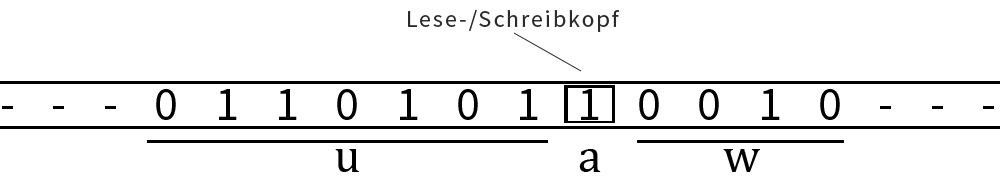
\includegraphics[width=0.85\linewidth]{./abbildungen/turing-snapshot}
	\end{center}

	\begin{itemize}
		\item Linkskontext: $u$
		\item Interner Zustand: $q$
		\item Gelesenes Symbol: $a$
		\item Rechtskontext: $w$
	\end{itemize}
	Somit lässt sich der Zustand $Q_t$ einer Turingmaschine zum Zeitpunkt $t$ durch die Folge $u_tq_ta_tw_t$ darstellen.
	\end{block}
} \frame {		
	\begin{block}{Rechenweg}
	Den Rechenweg einer Turingmaschine können wir als die Folge von Zuständen $Q_0, ..., Q_n$ vom Startzeitpunkt $t = 0$ bis zum Endzeitpunkt $t = n$ bei dem die Turingmaschine einen der Endzustände erreicht hat.
	% Formulierung überarbeiten 
	\end{block}
} \frame {	
	\begin{block}{Beispiel}
	Formalisierte Darstellung: $0110101q_010010\sharp01101011q_100010$ \newline
	Der Lesekopf liest eine $1$ und befindet sich in Zustand $q_0$, die Regel die Anwendung gefunden hat ist $q_01 \rightarrow q_10R$.
	\end{block}	
	\pause[2]
	\begin{block}{Simulation der Regel $q_10 \rightarrow q_11R$}
	$0110101q_010010\sharp01101011q_100010\sharp\pause[3]0\pause[4]1\pause[5]1\pause[6]0\pause[7]1\pause[8]0\pause[9]1\pause[10]1\pause[11]1q_1\pause[12]0\pause[13]010\pause[14]\sharp$\newline
	$\pause[2]0110101q_010010\sharp\pause[3]0\pause[4]1\pause[5]1\pause[6]0\pause[7]1\pause[8]0\pause[9]1\pause[10]1\pause[11]q_10\pause[12]0\pause[13]010\pause[14]\sharp$
	\end{block}
	
} \frame {
	\frametitle{Simulationsregeln}
	\textbf{1. Anfangsregel}
		\begin{tabbing}
			\kill
			$(\sharp\sharp q_0w\sharp, \sharp)$ 
		\end{tabbing} \pause
	\textbf{2. Kopierregeln} 
		\begin{tabbing}
			LinksNochWeiter \= Rechts \kill
			$(a, a)$ \> für alle $a \in \Gamma \cup \{\sharp\}$
		\end{tabbing} \pause	
	\textbf{3. Überführungsregeln} 
		\begin{tabbing}
			LinksNochWeiter \= Rechts \kill
			$(cq', qa)$ \> falls $qa \rightarrow q'cR$, für $q \in Q, a \in \Gamma$ \\
			
			$(q'bc, bqa)$ \> falls $qa \rightarrow q'cL$, für $q \in Q, a \in \Gamma$ 
		\end{tabbing} \pause	
	\textbf{4. Aufholregeln}
		\begin{tabbing}
			LinksNochWeiter \= Rechts \kill
			$(q, aq)$ \> für $a \in \Gamma$ und $q \in Q_f$ \\
			
			$(q, qa)$ \> für $a \in \Gamma$ und $q \in Q_f$
		\end{tabbing} \pause
	\textbf{5. Abschlussregel}
		\begin{tabbing}
			LinksNochWeiter \= Rechts \kill
			$(\sharp, q\sharp\sharp)$ \> für $q \in Q_f$ 
		\end{tabbing}
} \frame {
	\frametitle{Aufhol- und Abschlussregeln}
	
		\begin{block}{Aktuelle Situation}
		Aktueller Zustand der Turingmaschine: $0110101q_f10010$ \newline
		Die Turingmaschine ist in einem akzeptierenden Zustand $q_f$ angekommen.
		\end{block}	
		\pause[2]
		\begin{block}{Aufholen und Abschließen des PKPs}
		$0110101q_f10010\sharp\pause[3]0\pause[4]11010\pause[5]q_f\pause[6]1\pause[7]0010\sharp\pause[8]01101q_f10010\sharp\pause[9]0110q_f10010\sharp$\newline
		$\pause[3]0\pause[4]11010\pause[5]1q_f\pause[6]1\pause[7]0010\sharp\pause[8]011010q_f10010\sharp\pause[9]01101q_f10010\sharp$
		\end{block}

} \frame {
	\frametitle{Aufhol- und Abschlussregeln}
	
		\begin{block}{Aktuelle Situation}
		Aktueller Zustand der Turingmaschine: $0110101q_f10010$ \newline
		Die Turingmaschine ist in einem akzeptierenden Zustand $q_f$ angekommen.
		\end{block}	

		\begin{block}{Aufholen und Abschließen des PKPs}
		$0q_f10010\sharp\pause[2]q_f10010\sharp\pause[3]q_f0010\sharp\pause[4]q_f010\sharp\pause[5]q_f10\sharp\pause[6]q_f0\sharp\pause[7]q_f\sharp\pause[8]\sharp$\newline
		$\pause[2]0q_f10010\sharp\pause[3]q_f10010\sharp\pause[4]q_f0010\sharp\pause[5]q_f010\sharp\pause[6]q_f10\sharp\pause[7]q_f0\sharp\pause[8]q_f\sharp\sharp$
		\end{block}

}

\frame{
	\frametitle{Beweis der Nichtberechenbarkeit}
	
	\pause
	
	\begin{block}{Reduktion des Halteproblems auf das PKP:}
		Sei $M$ eine Turingmaschine und $w$ ihre Eingabe, so lässt sich das Halteproblem durch die Übergangsfunktion f auf das PKP reduzieren:
		 
		\[X_{Halte} (M, w) \Leftrightarrow X_{PKP}(f(M, w))\]
	\end{block}

	
	
	
	% % Halteproblem
	% % Reduktion
}

\frame{
	\frametitle{Beweise weiterer Probleme}
	Seien $G_1$ und $G_2$ zwei kontextfreie Grammatiken, und $L_1 = L(G_1)$ und $L_2 = L(G_2)$ zwei daraus konstruierte kontextfreie Sprachen.
	
	\begin{block}{Mehrdeutigkeitstest}
	Ist $G_1$ eindeutig?
	\end{block}
	
	\begin{block}{Gleichheitstest}
	Ist $L_1 = L_2$?
	\end{block}
}

\frame{
	\frametitle{Mehrdeutigkeitstest}
	
	\begin{block}{Konstruktion}
		Wir konstruieren eine kontextfreie Grammatik $G_x(V, \Sigma, P, S_x)$ mit $\{x_1, x_2, ..., x_n\} \in \Sigma$ und den zusätzlichen Symbolen $A = \{a_1, a_2, ..., a_k\} \notin \Sigma$ mit den Produktionen $P = \{S_x \rightarrow x_1 S_x a_1, ..., S_x \rightarrow x_n S_x a_n, S_x \rightarrow x_1 a_1, ... S_x \rightarrow x_n a_n\}$
		Zusätzlich konstruieren wir eine zweite Grammatik $G_y$ analog und eine Grammatik $G$ mit den Produktionsregeln $P = (S \rightarrow S_x, S \rightarrow S_y)$
	\end{block}
	\pause
	$G_x$ und $G_y$ sind offensichtlich eindeutig.
	
	$G$ ist dann mehrdeutig, wenn $G_x$ und $G_y$ mindestens ein gemeinsames Wort erzeugen. Dann hat das PKP $x_{i_k}...x_{i_1}a{i_1}...a{i_k} = y_{i_k}...y_{i_1}a{i_1}...a{i_k}$ mindestens eine Lösung mit der Indexfolge $I = {i_1, i_2, ... i_k}$.
	
	Somit lässt sich das PKP auf den Mehrdeutigkeitstest reduzieren, und der Mehrdeutigkeitstest ist folglich nicht berechenbar.
}

\frame{
	\frametitle{Gleichheitstest}
	
	% % Beweis
}

\frame{
	\frametitle{Vielen Dank für Ihre Aufmerksamkeit!}
}
\end{document}
